%%
%  ******************************************************************************
%  * #file    Szablon_raportu_EN_Latex.tex
%  * #author  Adrian Wójcik   adrian.wojcik(at)put.poznan.pl
%  *          
%  * #commit  Patryk Kościk   koscikpatryk(at)gmail.com
%  *          Modified the template for Projekt przejsciowy purposes          
%  *          
%  * #version 1.0
%  * #date    09-Mar-2022
%  * #brief   PROJPRZEJ
%  *
%  ******************************************************************************
%%  
\documentclass[11pt, a4paper]{article}

\usepackage{Szablon_raportu_EN_Latex}

% Wypełnijcie te dyrektywy zgodnie z waszym tematem
% \lab      -> NAZWA CZUJNIKA, np.: 'DHT22'
% \comment  -> Króciutki opis co to, np.: 'Cyfrowy budżetowy czujnik temperatury'
%
\lab{Moduł SE045}
\comment{Czujnik poziomu cieczy}
\author{Hubert Pietrzak}

% Absolutny zakaz dotykania tego tutaj bo jak dotkiecie to coś jebnie
\university{Politechnika Poznańska}
\faculty{Wydział Automatyki, Robotyki i Elektrotechniki}
\institute{Instytut Robotyki i Inteligencji Maszynowej}
\department{Zakład Sterowania i Elektroniki Przemysłowej}
\addbibresource{Szablon_raportu_EN_Latex.bib}
\nocite{*}


%%
%
% Początek dokumentu
%
%%
\begin{document}

%% Strona tytułowa %%
\mainpage{Czunik_back}
\newpage

\section*{Opis elementu} \addcontentsline{toc}{section}{Wstęp}


Czujnik służacy do wyznaczenia poziomu cieczy (na przykład wody) w naczyniu. Zasilay jest napięciem 5.0V. Wyjściem jest analogowe napięcie, które zwiększa swoją wartość (do 3.5V) wraz z głębokością zanużenia sondy czujnika. Sonda pomiarowa zbiera dane do 40mm głębokości.



\vspace{0.5cm}
\begin{figure}[h]
\centering
\begin{subfigure}{.5\textwidth}
  \centering
  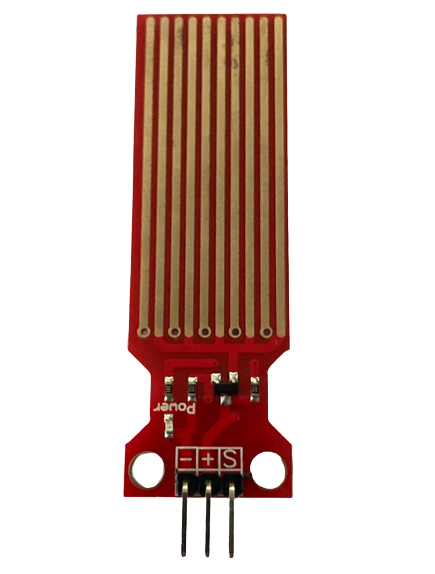
\includegraphics[width=.5\linewidth]{fig/obrazki/zdj_modułu/Czunik_back.png}
  \caption{Czujnik poziomu cieczy - przód}
  \label{fig:sub1}
\end{subfigure}%
\begin{subfigure}{.5\textwidth}
  \centering
  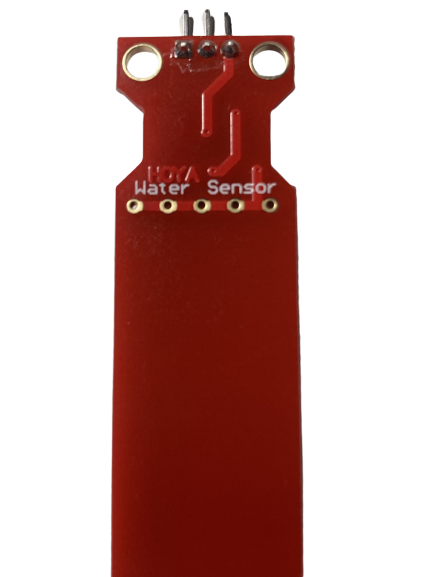
\includegraphics[width=.45\linewidth]{fig/obrazki/zdj_modułu/IMG-3416-removebg-preview.png}
  \caption{Czujnik poziomu cieczy - tył}
  \label{fig:sub2}
\end{subfigure}
\caption{Czujnik poziomu cieczy - zdjęcia poglądowe}
\label{fig:test}
\end{figure}
\vspace{0.5cm}

%\subsection{Zasada działania}

W czujniku poziomu wody mamy trzy wyprowadzenia pin. Zasilanie "$+$", masę GND oraz wyjście analogowe \textbf{S} które podłączamy do wyprowadzenia przetwornika A/C w naszym mikrokontrolerze (ponieważ z przetwornika odczytywana jest wartość napięcia z Analog Output czujnika).Po podłaczeniu urządzenia, poprzez diodę LED mamy informację o działaniu sensora.
Mikrokontroler odczytuje wartość w zakresie od 0 do 1023 w zależności od głębokości położenia sondy, która jest jednym z elementów modułu. Dzięki tranzystorowi J3Y typu n-p-n sterujemy prądem bazy by otwierać i zamykać przepływ prądu z kolektora do emitera, z którego to otrzymujemy dany poziom zanurzenia sondy w cieczy.

\vspace{0.5cm}
\begin{figure}[h]
  \centering
  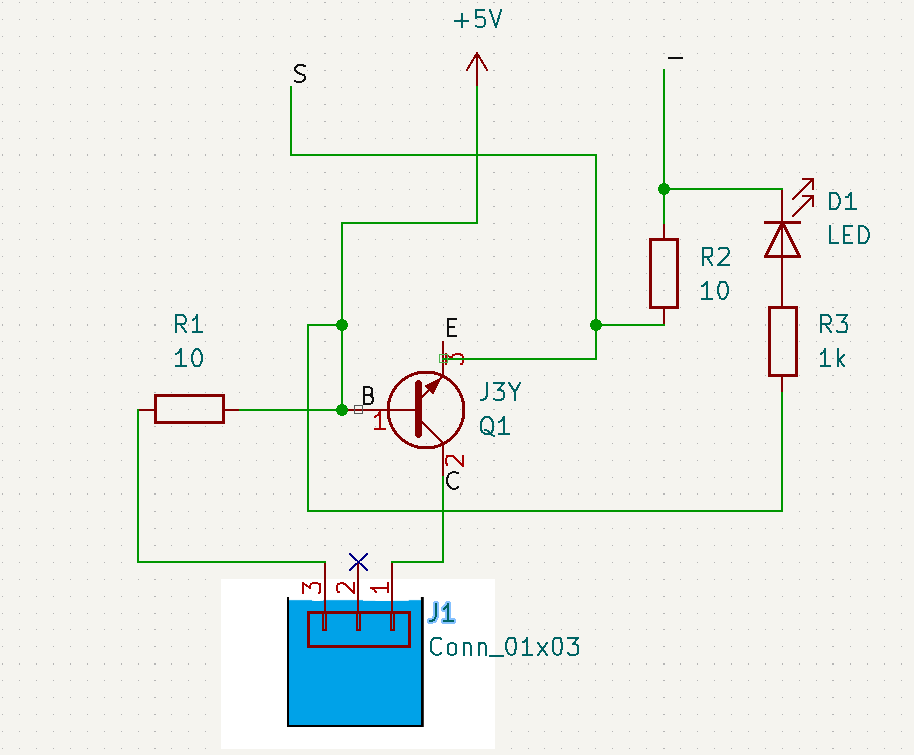
\includegraphics[width=.55\linewidth]{fig/obrazki/zasada_dzialania/KICAD.png}  
  \caption{Schemat}
  \label{fig:sub1}
\end{figure}


%\subsection{Zastosowania}



\newpage

%\section{Implementacja czujnika}


% \vspace{0.5cm}

% \vspace{0.5cm}
% \begin{figure}[h!]
%     \centering
%     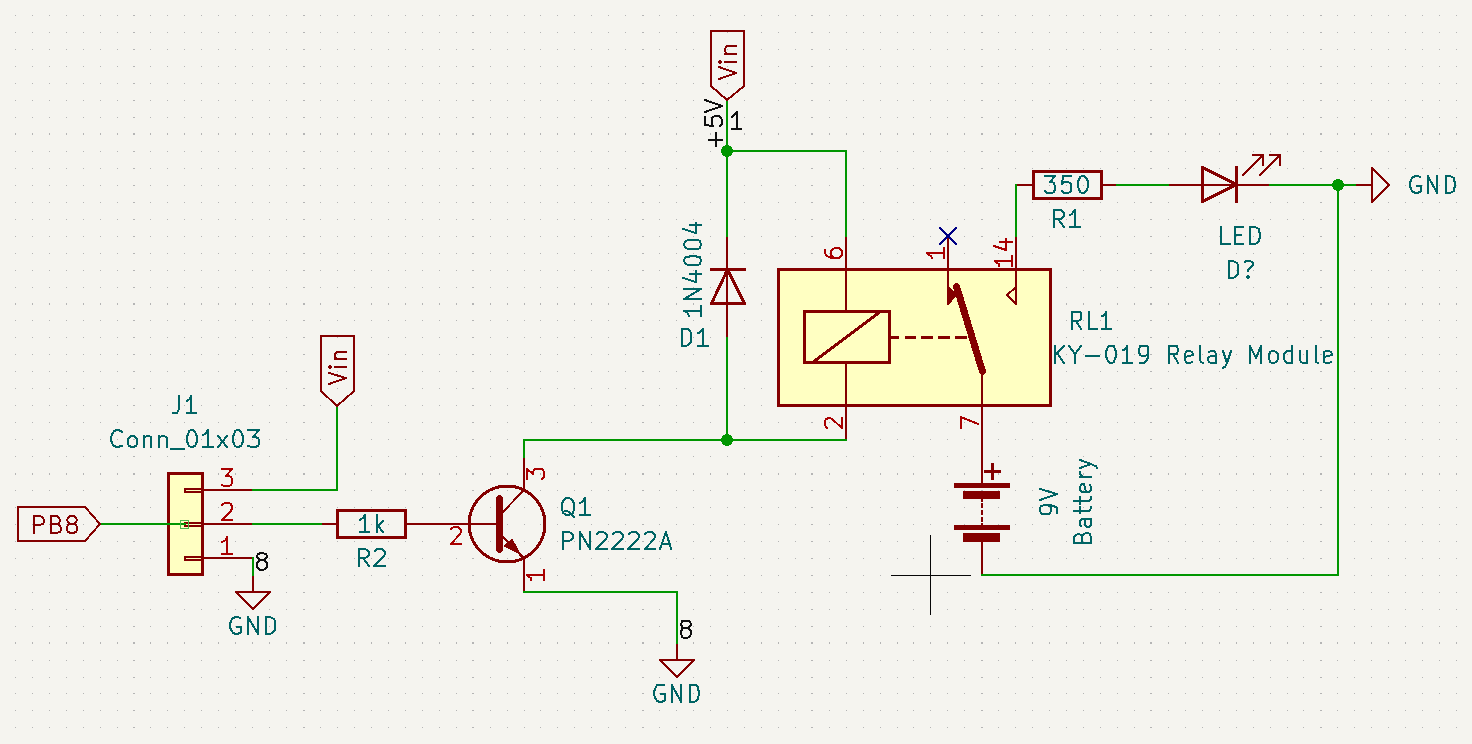
\includegraphics[scale=0.53]{fig/obrazki/polaczenie_modulu/Schematki.png}
%     \caption{Połaczenie elektryczne}
%     \label{fig:my_label}
% \end{figure}
% \vspace{0.5cm}


\newpage

%\section{Prezentacja działania układu}
\section{Użycie czujnika}

% \vspace{0.5cm}
% \begin{figure}[h!]
%     \centering
%     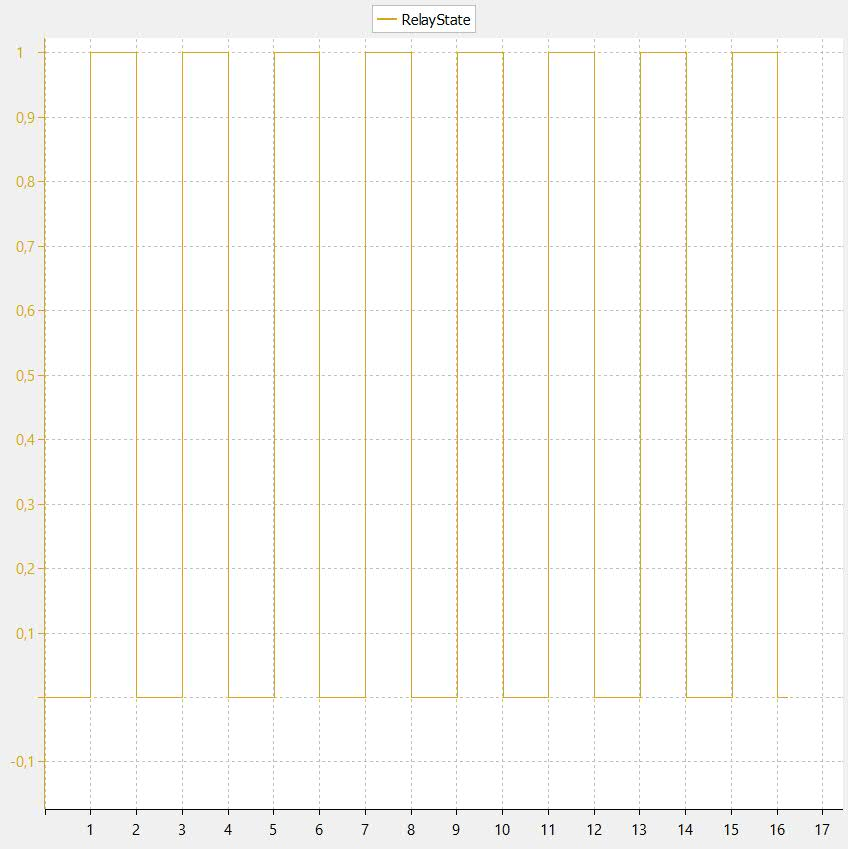
\includegraphics[width=0.6\textwidth]{fig/obrazki/działanie_ukladu/SWV.jpeg}
%     \caption{Przykładowy zrzut ekranu z SWV}
%     \label{fig:my_label}
% \end{figure}
% \vspace{0.5cm}


Do prezentacji podstawowej funkcjonalności czujnika wykorzystana zostało NUCLEO F746ZG, układ został podłączony do zasilania oraz do wcześniej skonfigurowanego wyprowadzenia na płytce mikrokontrolera (włączenie przetwornika A/C dla tego konkretnego pinu). Dodatkowo w celu prezentacji wykorzystana została szklanka z woda w środku. Obserować możemy trzy stany zanurzenia sensora:
\begin{itemize}
    \item Lekkie zanurzenie - zaprogramowane w ten sposób by zapalała się dioda  LD1 (zielona) określająca niski stan zanurzenia (niewielki sygnał napięciowy)
    \item Średnie zanurzenie - zapala się dioda LD2 (niebieska)
    \item Głębokie zanurzenie - zapala się dioda LD3 (czerwona)
\end{itemize}

Należy pamiętać, że w przypadku głębszego zanurzenia sondy napięcie rośnie ( do 3.5V).
Wszystkie stany pośrednie można zaobserwować na poniższych fotografiach oraz na filmiku prezentacyjnym zamieszczonym w bibliografii.


\vspace{0.5cm}
\begin{figure}[h!]
    \centering
    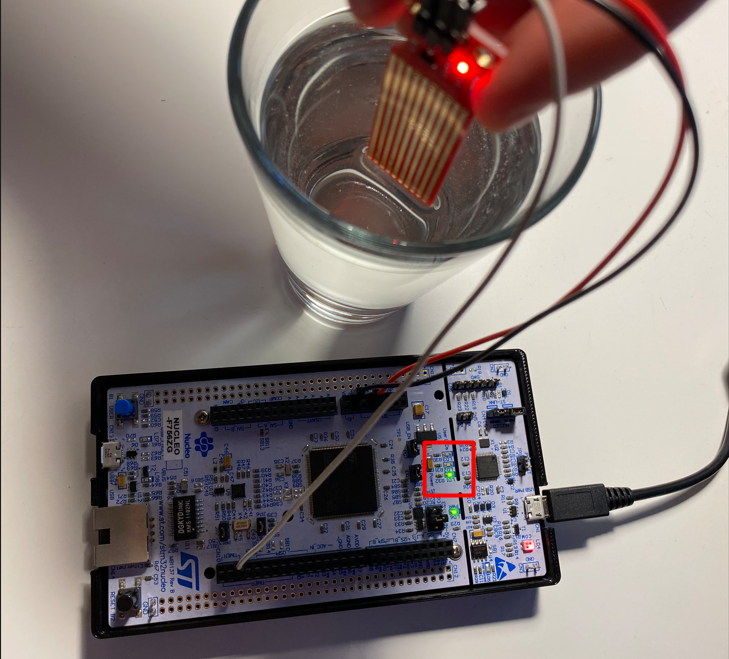
\includegraphics[scale=0.75]{fig/obrazki/działanie_ukladu/zielony.png}
    \caption{Lekkie zanurzenie}
    \label{fig:my_label}
\end{figure}
\vspace{0.5cm}



\vspace{0.5cm}
\begin{figure}[h!]
    \centering
    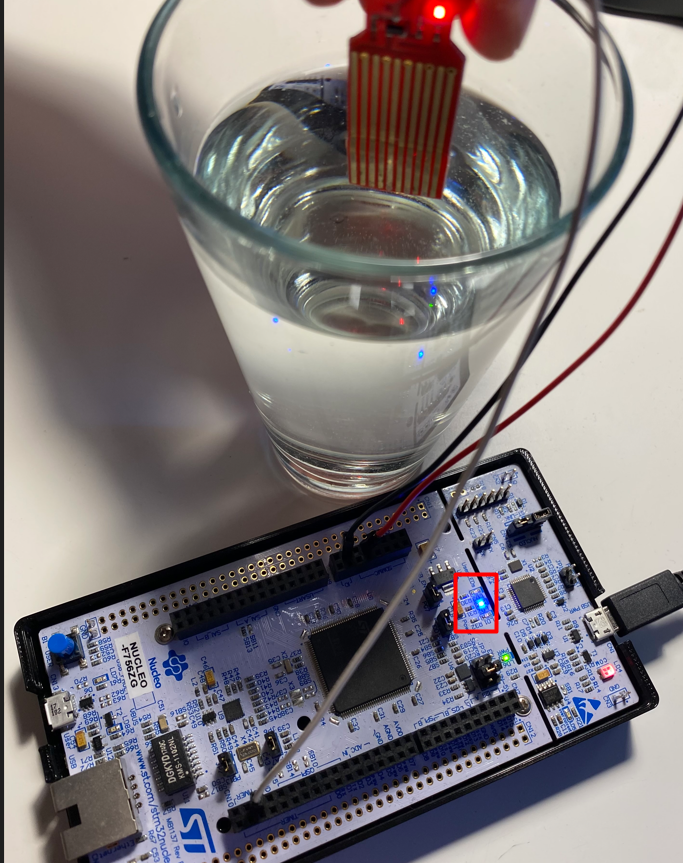
\includegraphics[scale=0.6]{fig/obrazki/działanie_ukladu/niebieski.png}
    \caption{Średni poziom zanurzenia}
    \label{fig:my_label}
\end{figure}
\vspace{0.5cm}



\vspace{0.5cm}
\begin{figure}[h!]
    \centering
    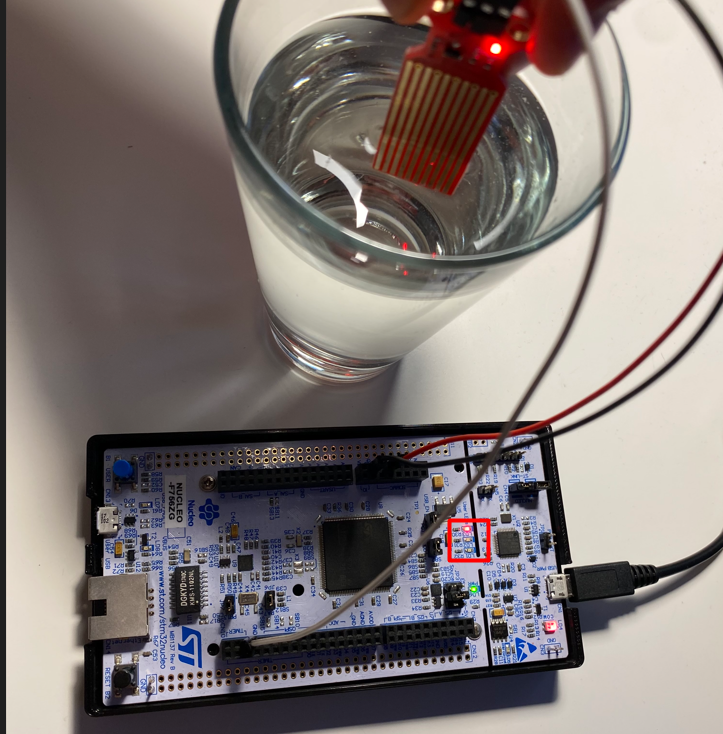
\includegraphics[scale=0.6]{fig/obrazki/działanie_ukladu/czerwony.png}
    \caption{Głębokie zanurzenie}
    \label{fig:my_label}
\end{figure}
\vspace{0.5cm}





\section*{Podsumowanie} \addcontentsline{toc}{section}{Podsumowanie}
Czujnik poziomu cieczy jest sensorem, który kontroluje poziom zanurzenia się sondy w cieczy (między innymi wodzie), podaje na wyjściu proporcjonalny sygnału napięciowy, by poprzez przetwornik analgowo-cyfrowy, został on odczytany w sposób czytelny dla mikrokontrolera (cyfrowo).
\printbibliography[heading=bibintoc]

\end{document}